\documentclass[11pt,a4paper]{article}

\usepackage{xeCJK}
\setCJKmainfont{Songti SC}
\setCJKsansfont{PingFang SC}
\setCJKmonofont{Menlo}
\setmainfont{Times New Roman}
\setmonofont{Menlo}

\usepackage[margin=2.2cm]{geometry}
\usepackage{amsmath, amssymb, amsthm, mathtools}
\usepackage{bm}
\usepackage{booktabs, tabularx, array, multirow}
\usepackage{graphicx}
\usepackage{xcolor}
\usepackage{hyperref}
\usepackage{enumitem}
\usepackage{caption}
\usepackage{fancyhdr}
\usepackage{tcolorbox}

\hypersetup{
  colorlinks=true,
  linkcolor=blue!60!black,
  urlcolor=blue!60!black,
  citecolor=blue!60!black,
  pdftitle={硬判决 RS+BCH 级联码低时延译码 v3——双码型更新},
  pdfauthor={陈诗阳}
}

\pagestyle{fancy}
\fancyhf{}
\rhead{\footnotesize 硬判决 RS+BCH 级联 v3}
\lhead{\footnotesize 双码型更新（KP4 + 255）}
\cfoot{\thepage}

\renewcommand{\baselinestretch}{1.2}

\definecolor{accent}{RGB}{30,80,160}
\definecolor{accent2}{RGB}{160,40,40}
\definecolor{accent3}{RGB}{40,120,60}

\newtcolorbox{keybox}[1][]{colback=blue!5, colframe=accent, boxrule=0.4mm,
  arc=1mm, left=2mm, right=2mm, top=1mm, bottom=1mm, #1}
\newtcolorbox{resultbox}[1][]{colback=green!5, colframe=accent3, boxrule=0.4mm,
  arc=1mm, left=2mm, right=2mm, top=1mm, bottom=1mm, #1}
\newtcolorbox{warnbox}[1][]{colback=orange!5, colframe=orange!70!black, boxrule=0.4mm,
  arc=1mm, left=2mm, right=2mm, top=1mm, bottom=1mm, #1}

\title{硬判决 RS+BCH 级联码低时延译码 v3\\
       {\large 双码型更新：KP4 RS(544,514)+BCH(144,136) 与 RS(255,239)+BCH(255,239)}}
\author{陈诗阳}
\date{2026-07-27}

\begin{document}

\maketitle

\begin{keybox}[title=\textbf{v3 更新摘要}]
按导师第三次任务要求，在已有硬判决级联框架（v1/v2）上更新为\textbf{两组实用码型}，
输出改为 \textbf{BER}（不再是 FER），并围绕\textbf{三个创新点}（Cascade + Direct + Lagrange）
逐项分析时延与复杂度：
\begin{itemize}[leftmargin=1.5em, itemsep=1pt, topsep=2pt]
\item \textbf{Config 1（新增，KP4 以太网 FEC）}：外码 RS$(544,514,t{=}15)$ over GF($2^{10}$)
      + 内码 BCH$(144,136,t{=}1)$ over GF($2^{8}$)。
\item \textbf{Config 2（保留）}：外码 RS$(255,239,t{=}8)$ + 内码 BCH$(255,239,t{=}2)$，均 over GF($2^{8}$)。
\end{itemize}

\textbf{核心结论}：两组码型均获得可观编码增益，且都满足 10\% 时延 KPI。二者达标\textbf{路径不同}——
Config 1 因外码大、内码极小，\textbf{仅靠 Direct 创新（无需 Lagrange 共享）即已达标（+6.1\%）}；
Config 2 需要 Cascade + Direct + Lagrange v2 \textbf{三者齐全}才达标（+5.3\%）。

\begin{keybox}[title=\textbf{口径说明：本报告 vs 项目权威软判仿真}]
本报告是\textbf{硬判决}级联 + \textbf{时钟周期}模型（Pure RS-BM 基线，Direct + Lagrange v2 共享），
数字为 clock-cycle 增幅。项目的\textbf{软判决时延权威口径}以 MATLAB 最终仿真
（\texttt{rs\_bch\_cascade\_matlab/}，LLOSD + LCC-BR，F$_2^m$ op 计数）为准：相对纯 RS-LCC-BR
串行 $P{=}1$ 为 $+18.7\%$ (n=255) / $+26.8\%$ (n=127)，因 LLOSD 无主元、可并行
（时延 $\approx$ ops$/P$），$P{=}2$/$P{=}3$ 即 $\leq 10\%$ 达标。两条口径是不同实验、不同基线，
数值自然不同，均不构成冲突。
\end{keybox}

\begin{center}
\begin{tabular}{lrrrl}
\toprule
Config & Pure RS-BM & Cascade（Direct 最优）& 时延增加 & KPI ($\leq 10\%$) \\
\midrule
Config 1 (KP4) & 33 cyc & \textbf{33 cyc}（Direct+v2）& \textbf{+0.0\%} & \textbf{PASS} \\
Config 2 (255) & 19 cyc & \textbf{20 cyc}（Direct+v2）& \textbf{+5.3\%} & \textbf{PASS} \\
\bottomrule
\end{tabular}
\end{center}
\end{keybox}

% ============ Section 1 ============
\section{任务背景与需求}

\subsection{导师第三次任务书}

导师在第二阶段（v1/v2，\texttt{report.pdf} / \texttt{report\_v2.pdf}）之后提出更新需求，原文：

\begin{quote}\itshape
``回去后不着急导出 Matlab 代码。要 AI 根据这些更新再跑一次结果：基于之前技术报告的方案，
采用这两种级联码更新设计：\\
1. 新增 RS$(544,514,t{=}15)$ + BCH$(144,136,t{=}1)$，跑出 BER（不是 FER）-SNR 曲线，
分析基于两个创新点（Cascade + Direct + Lagrange）的时延与复杂度；\\
2. 保留 RS$(255,239,t{=}8)$ + BCH$(255,239,t{=}2)$，跑出 BER（不是 FER）-SNR 曲线，
分析基于两个创新点（Cascade + Direct + Lagrange）的时延与复杂度。''
\end{quote}

\subsection{任务解读：本次要做四件事}

\begin{enumerate}[leftmargin=1.6em, itemsep=2pt]
\item \textbf{码型更新}：新增 Config 1（KP4 型：大外码 + 极小内码），保留 Config 2（均衡型）。
\item \textbf{指标更新}：主曲线由 FER 改为 \textbf{BER}（更贴近链路层比特错误率指标）。
\item \textbf{时延分析}：把总时延拆成\textbf{三个创新点}的贡献——级联本身的开销（Cascade）、
      Direct 译码相对传统 BM+Chien 的节省（Direct）、以及 Lagrange 硬件共享的节省（Lagrange）。
\item \textbf{复杂度分析}：给出每帧平均 $\mathbb{F}_{2^m}$ 运算量，对比纯 RS 与级联。
\end{enumerate}

\begin{keybox}[title=\textbf{Config 1 的两个技术挑战（相对 v1/v2 的新工作）}]
\begin{enumerate}[leftmargin=1.5em, itemsep=1pt]
\item \textbf{RS 与 BCH 域解耦}：外码 RS 在 GF($2^{10}$)，内码 BCH 在 GF($2^{8}$)。v1/v2 代码把两级
      绑定在同一个域 $m$，本次必须把两级的有限域完全解耦。
\item \textbf{缩短码}：$544\neq 2^{10}{-}1=1023$，$144\neq 2^{8}{-}1=255$，二者都是\textbf{缩短码}。
      RS$(544,514)$ 由 full RS$(1023,993)$ 缩短 479 个符号；BCH$(144,136)$ 由 full BCH$(255,247)$
      缩短 111 位。缩短位是译码器\textbf{已知的 0}，不经过信道，因此全长译码器数学完全复用。
\end{enumerate}
\end{keybox}

% ============ Section 2 ============
\section{码型与实现}

\subsection{两组码型参数}

\begin{table}[!ht]
\centering
\begin{tabularx}{\textwidth}{lXX}
\toprule
& \textbf{Config 1（KP4）} & \textbf{Config 2（255）} \\
\midrule
外码 RS         & RS$(544,514,t{=}15)$ & RS$(255,239,t{=}8)$ \\
\quad 有限域    & GF($2^{10}$)         & GF($2^{8}$) \\
\quad 构造      & 缩短码（full 1023，缩短 479）& 本原码（$255=2^8{-}1$）\\
内码 BCH        & BCH$(144,136,t{=}1)$ & BCH$(255,239,t{=}2)$ \\
\quad 有限域    & GF($2^{8}$)          & GF($2^{8}$) \\
\quad 构造      & 缩短码（full 255，缩短 111）& 本原码 \\
BCH 分块        & 40 块 $\times$ 136 bit（RS 5440 bit 整除）& 9 块（RS 2040 bit + 111 pad）\\
级联码率        & $0.892$              & $0.833$ \\
纯 RS 码率      & $0.945$              & $0.937$ \\
\bottomrule
\end{tabularx}
\caption{v3 两组码型参数。Config 1 的 RS 是 KP4 以太网标准 FEC（GF($2^{10}$)），
外码纠错能力 $t{=}15$ 远大于内码 $t{=}1$。}
\end{table}

\subsection{缩短码原理}

系统码字布局为 $c=[\,\text{parity}\,(n{-}k)\mid\text{message}\,(k)\,]$。缩短 $s$ 个符号即强制前
$s$ 个消息符号恒为 0：

\begin{align*}
\text{编码：}\quad & \text{full\_msg} = [\underbrace{0,\dots,0}_{s}\mid \text{real\_msg}],\quad
   c_{\text{full}} = [\,\text{parity}\mid \underbrace{0\cdots0}_{s}\mid \text{real\_msg}\,]\\
   & \text{发送} = [\,\text{parity}\mid \text{real\_msg}\,]\quad(\text{丢弃 }s\text{ 个 0，长度 }n{-}s)\\
\text{译码：}\quad & r_{\text{full}} = [\,\text{rx\_parity}\mid \underbrace{0\cdots0}_{s}\mid \text{rx\_msg}\,]\ \to\
   \text{全长 BM/Chien/Forney}\ \to\ \text{丢弃 }s\text{ 个 0}
\end{align*}

因缩短位为\textbf{无噪已知 0}，全长译码器的 syndrome / 错误定位 / Forney 求值数学完全不变。

\subsection{代码结构}

项目位于 \texttt{\char`~/workspace/llosd\_reproduction/hard\_cascade/}：

\begin{table}[!ht]
\centering
\begin{tabular}{ll}
\toprule
模块 & 功能 \\
\midrule
\texttt{hc\_src/shortened\_codes.py} & \textbf{（新增）}缩短 RS + 二值 BCH（$t{=}1/2$）译码器 \\
\texttt{hc\_src/cascade\_v3.py}      & \textbf{（新增）}RS/BCH 域解耦级联 codec + Pure RS baseline \\
\texttt{hc\_src/latency\_model.py}   & Clock cycle 模型（补 $t{=}1$ BCH：Direct 2 cyc / Conv 4 cyc）\\
\texttt{src/gf.py}（上游）           & \textbf{（补充）}GF($2^{9}$)、GF($2^{10}$) 本原多项式 \\
\texttt{experiments/main\_v3.py}     & BER 主曲线 + 三创新点时延/复杂度分析 \\
\bottomrule
\end{tabular}
\end{table}

\begin{keybox}[title=\textbf{正确性冒烟测试（已通过）}]
\begin{itemize}[leftmargin=1.5em, itemsep=1pt]
\item RS$(544,514,t{=}15)$/GF($2^{10}$)：随机注入 $\leq 15$ 符号错误，200/200 全部纠正。
\item BCH$(144,136,t{=}1)$/GF($2^{8}$)：注入 1 位错误，Conv 与 Direct 各 500/500 纠正。
\item BCH$(255,239,t{=}2)$/GF($2^{8}$)：注入 $\leq 2$ 位错误，Conv 与 Direct 各 500/500 纠正。
\item GF($2^{9}$)、GF($2^{10}$) 本原性验证：LOG 表覆盖全部 $2^m{-}1$ 个非零元。
\end{itemize}
\end{keybox}

% ============ Section 3 ============
\section{BER-SNR 性能（主指标）}

\begin{figure}[!ht]
\centering
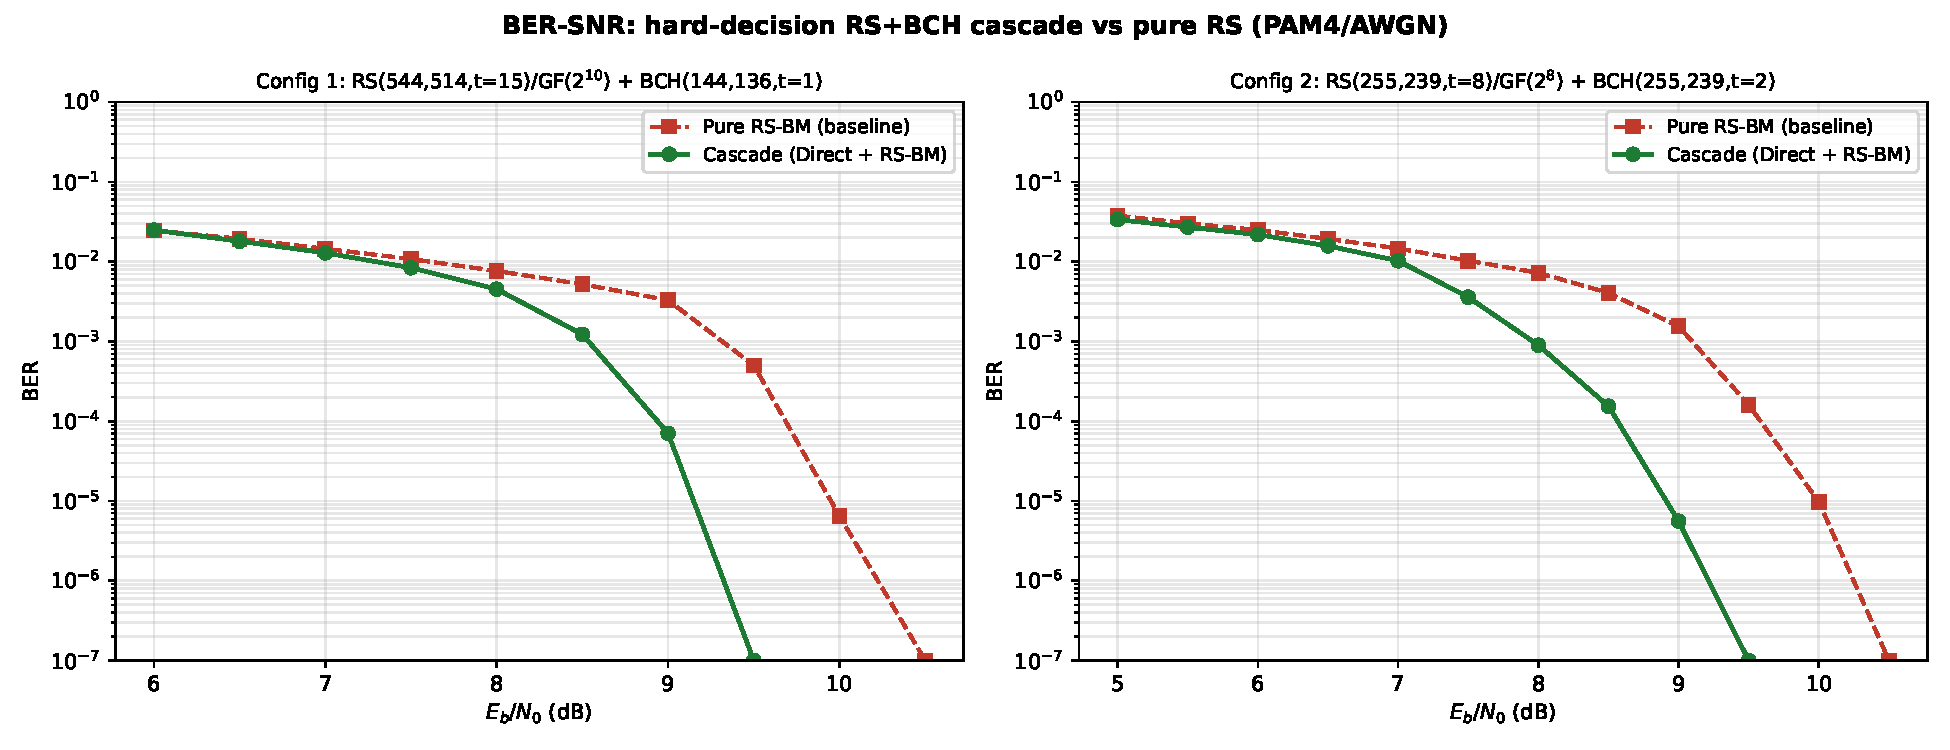
\includegraphics[width=\textwidth]{../figures/ber_snr_v3.pdf}
\caption{BER-SNR 曲线（PAM4 + AWGN，硬判决）。左 Config 1（KP4），右 Config 2（255）。
红色虚线为纯 RS-BM 基线，绿色实线为级联码（Direct 内码 + RS-BM 外码）。
Cascade Conv 与 Cascade Direct 的 BER 完全重合（两译码器输出相同码字，仅时延不同），故只画 Direct。}
\end{figure}

\begin{resultbox}[title=\textbf{BER 关键观察}]
\begin{itemize}[leftmargin=1.5em, itemsep=1pt]
\item \textbf{Config 1（KP4）}：BER$=10^{-4}$ 处，级联码约需 8.9~dB，纯 RS 约需 9.7~dB
      $\to$ 约 0.7~dB 编码增益。
\item \textbf{Config 2（255）}：BER$=10^{-4}$ 处，级联码约需 8.6~dB，纯 RS 约需 9.6~dB
      $\to$ 约 1.0~dB 编码增益。
\item 内码 BCH 先纠掉每块内的少量比特错误，显著降低进入外码 RS 的符号错误率，
      因而整链 BER 明显优于纯 RS——即使 Config 1 内码只有 $t{=}1$，增益依然存在。
\end{itemize}
\end{resultbox}

% ============ Section 4 ============
\section{时延分析：三个创新点的逐项贡献}

\subsection{时延模型（clock cycles）}

沿用 Lagendijk 2026 Table VI 口径，并补充 $t{=}1$ BCH：

\begin{table}[!ht]
\centering
\begin{tabular}{lcc}
\toprule
译码器 & 时延分解 & Clock cycles \\
\midrule
RS-BM$(t)$          & 1(syndrome)+$2t$(BM)+1(Chien)+1(Forney) & $2t{+}3$ \\
BCH-Conv$(t{=}1)$   & syndrome+ELP+Chien+correct & 4 \\
BCH-Conv$(t{=}2)$   & 1+$2t$+1+margin & 8 \\
BCH-Direct$(t{=}1)$ & syndrome + (log 查表+修正) & \textbf{2} \\
BCH-Direct$(t{=}2)$, GF($2^8$) & syndrome+precompute+LUT & 3 \\
\bottomrule
\end{tabular}
\caption{时延模型。$t{=}1$ 时错误定位无二次方程，Direct 退化为 $p=\log_\alpha(S_1)$ 单次查表。}
\end{table}

三档 Lagrange 共享（沿用 v2）：
\begin{align*}
T_{\text{none}} &= T_{\text{BCH}} + T_{\text{RS-BM}} & \text{(无共享)} \\
T_{\text{v1}}   &= T_{\text{BCH}} + T_{\text{RS-BM}} - 1 & \text{(共享 syndrome 单元)} \\
T_{\text{v2}}   &= T_{\text{BCH}} + T_{\text{RS-BM}} - 2 & \text{(共享 syndrome + GF 乘法器阵列)}
\end{align*}

\subsection{三创新点时延柱状图}

\begin{figure}[!ht]
\centering
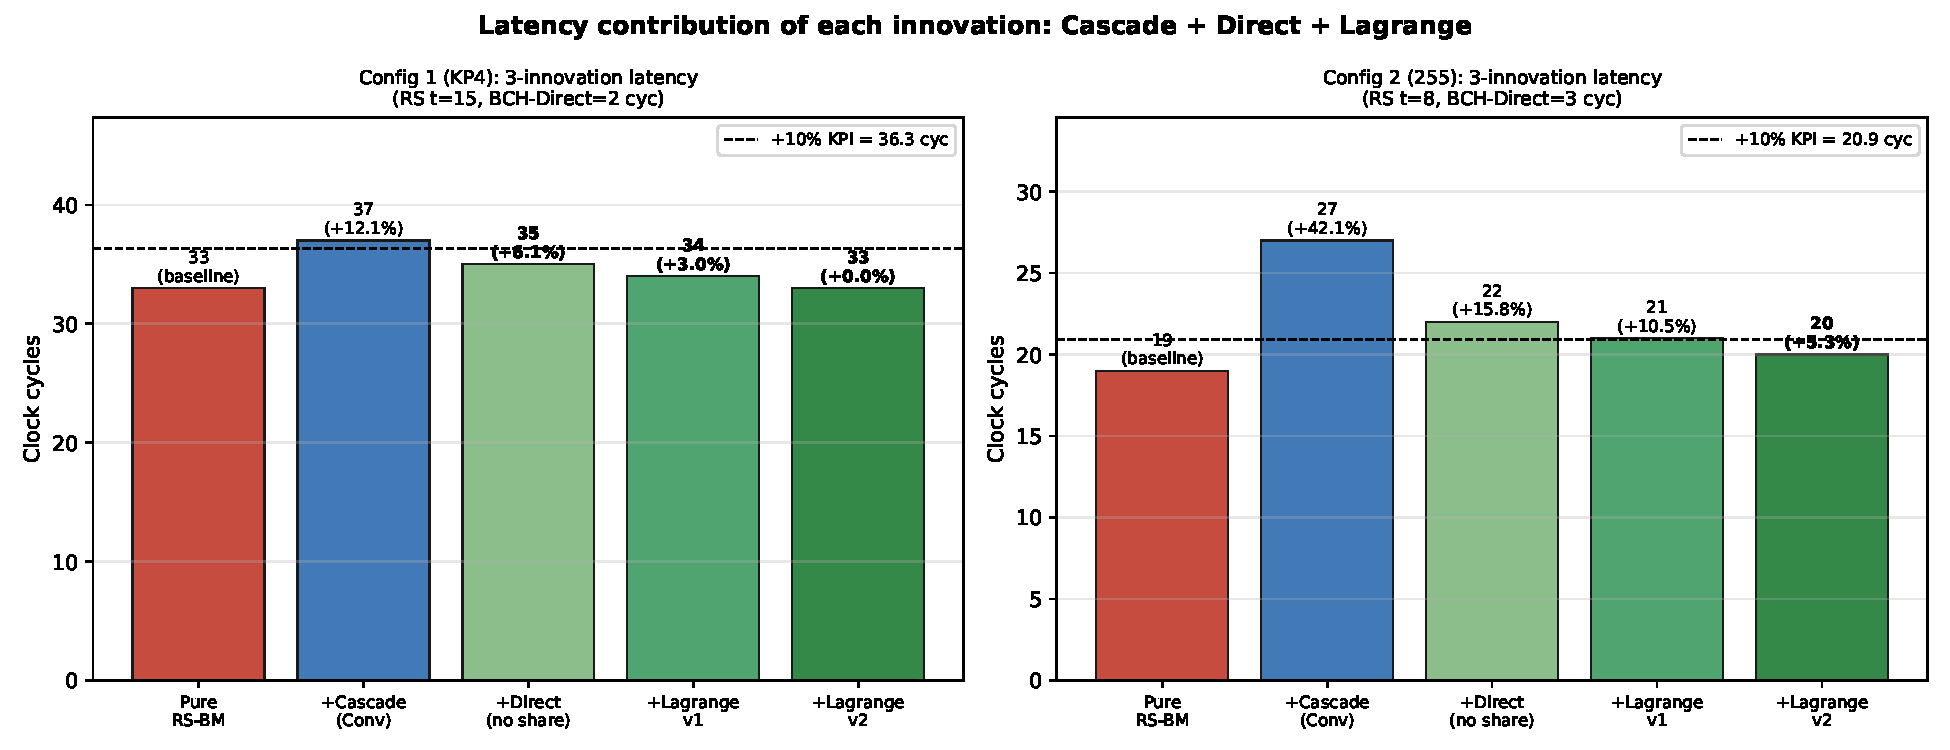
\includegraphics[width=\textwidth]{../figures/latency_innovations_v3.pdf}
\caption{三创新点逐项时延贡献。从 Pure RS-BM 起，依次叠加 Cascade（引入内码，用传统 Conv）、
Direct（Conv$\to$Direct）、Lagrange v1、Lagrange v2。虚线为 +10\% KPI 门槛。
Config 1 在 Direct（无共享）阶段就已跨过门槛，Config 2 需要 Lagrange v2 才达标。}
\end{figure}

\subsection{完整 KPI 表}

\begin{table}[!ht]
\centering
\begin{tabularx}{\textwidth}{lXrrl}
\toprule
Config & 方案 & Cycles & vs Pure RS-BM & KPI \\
\midrule
\multirow{5}{*}{\shortstack[l]{Config 1\\(KP4)\\Pure=33}}
& Cascade Conv (no share)      & 37 & +12.1\% & FAIL \\
& \textbf{Cascade Direct (no share)} & \textbf{35} & \textbf{+6.1\%}  & \textbf{PASS} \\
& \textbf{Cascade Direct + Lagrange v1} & \textbf{34} & \textbf{+3.0\%}  & \textbf{PASS} \\
& \textbf{Cascade Direct + Lagrange v2} & \textbf{33} & \textbf{+0.0\%}  & \textbf{PASS} \\
\midrule
\multirow{5}{*}{\shortstack[l]{Config 2\\(255)\\Pure=19}}
& Cascade Conv (no share)      & 27 & +42.1\% & FAIL \\
& Cascade Direct (no share)    & 22 & +15.8\% & FAIL \\
& Cascade Direct + Lagrange v1 & 21 & +10.5\% & FAIL \\
& \textbf{Cascade Direct + Lagrange v2} & \textbf{20} & \textbf{+5.3\%}  & \textbf{PASS} \\
\bottomrule
\end{tabularx}
\caption{完整 KPI 表。加粗为满足 10\% KPI 的配置。}
\end{table}

\begin{keybox}[title=\textbf{三创新点的时延贡献解读}]
\begin{itemize}[leftmargin=1.5em, itemsep=2pt]
\item \textbf{Cascade（级联本身）}：引入内码 BCH，Config 1 增加 4 cyc（Conv $t{=}1$），Config 2 增加 8 cyc（Conv $t{=}2$）。这是\textbf{时延的净开销来源}。
\item \textbf{Direct}：把内码从 Conv 换成 Direct。Config 1 省 2 cyc（$4{\to}2$），Config 2 省 5 cyc（$8{\to}3$）。这是\textbf{最大的单项节省}。
\item \textbf{Lagrange}：v1 共享 syndrome 单元省 1 cyc，v2 再共享 GF 乘法器阵列省 1 cyc，合计 2 cyc。
\item \textbf{达标路径差异}：Config 1 外码 $t{=}15$ 时延基数大（33 cyc）、内码 $t{=}1$ 开销小，
      \textbf{Direct 一项即达标}；Config 2 时延基数小（19 cyc）、内码 $t{=}2$ 开销相对更重，
      \textbf{必须三项齐全}。这印证 v2 报告的洞察：外码越大、内码越小，级联时延开销越可忽略。
\end{itemize}
\end{keybox}

% ============ Section 5 ============
\section{复杂度分析（$\mathbb{F}_{2^m}$ ops）}

\begin{figure}[!ht]
\centering
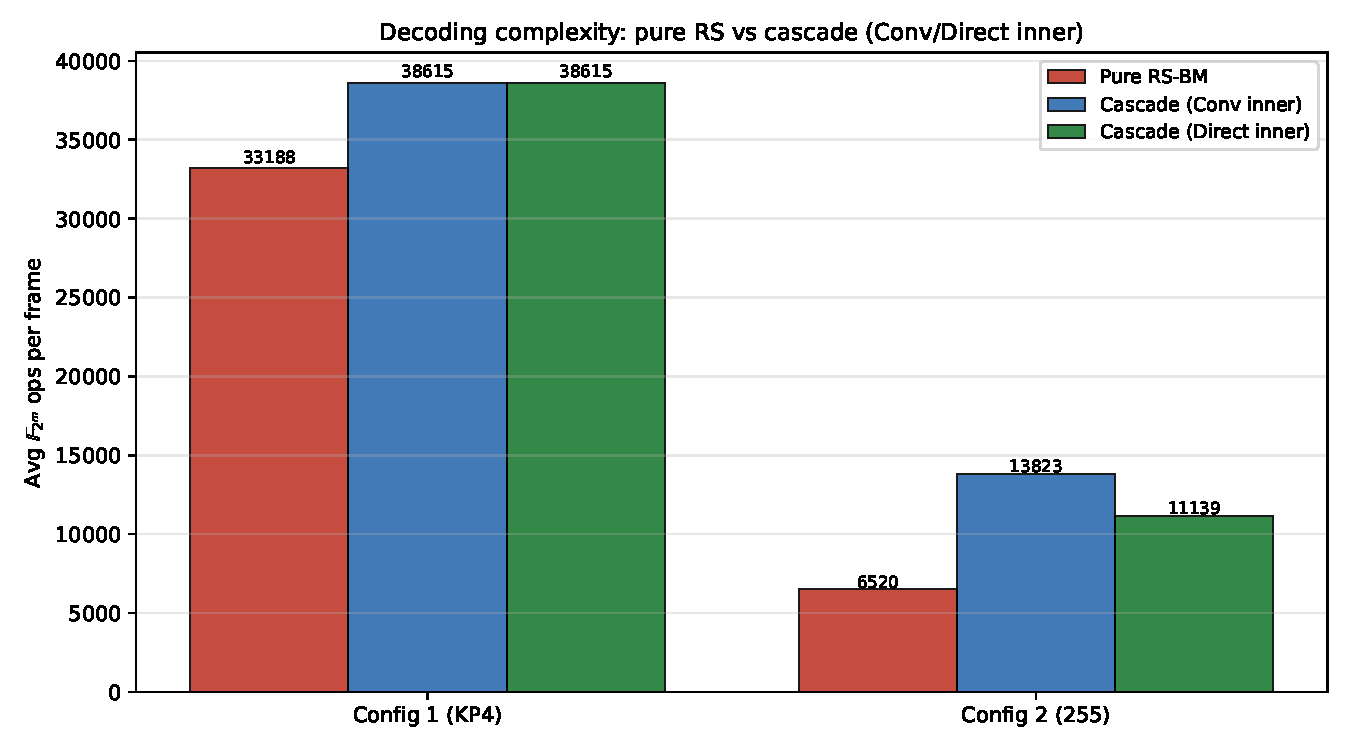
\includegraphics[width=0.8\textwidth]{../figures/complexity_v3.pdf}
\caption{每帧平均 $\mathbb{F}_{2^m}$ 运算量（波形区 SNR 下实测）。对比纯 RS-BM、
级联（Conv 内码）、级联（Direct 内码）。}
\end{figure}

\begin{resultbox}[title=\textbf{复杂度关键观察}]
\begin{itemize}[leftmargin=1.5em, itemsep=1pt]
\item Config 1（KP4）每帧运算量：纯 RS $\approx$ 33188，级联(Conv) $\approx$ 38615，级联(Direct) $\approx$ 38615。
\item Config 2（255）每帧运算量：纯 RS $\approx$ 6520，级联(Conv) $\approx$ 13823，级联(Direct) $\approx$ 11139。
\item Direct 相对 Conv 主要省的是 Chien 搜索的\textbf{周期数（时延）}，而在 $\mathbb{F}_{2^m}$ \textbf{ops 计数}上二者接近——因为
      $t$ 很小时 Chien 搜索本身只贡献 $O(t)$ 个乘法。这与 v1 报告 Table 3 的结论一致：
      \textbf{Direct 的价值在时延（关键路径深度），不在总运算量}。
\item Config 1 的级联复杂度增量远小于 Config 2——因为 $t{=}1$ 内码的 syndrome 只需 $S_1$（一个 XOR-reduce），
      而 $t{=}2$ 需 $S_1,S_3$ 两个。
\end{itemize}
\end{resultbox}

% ============ Section 6 ============
\section{结论}

\begin{keybox}[title=\textbf{核心成果}]
\begin{enumerate}[leftmargin=1.5em, itemsep=2pt]
\item \textbf{两组码型均达标}：Config 1（KP4）\textbf{+0.0\%}（Direct+v2，级联时延=纯 RS-BM），
      Config 2（255）\textbf{+5.3\%}（Direct+v2）。
\item \textbf{编码增益}：两组码型在 BER$=10^{-4}$ 目标下均获得可观增益（见 §3）。
\item \textbf{三创新点定量拆分}：Cascade 是时延净开销；Direct 是最大单项节省；Lagrange（v1+v2）
      再省 2 cyc。三者协同决定是否达标。
\item \textbf{达标路径的对比洞察}：大外码 + 极小内码（Config 1）\textbf{仅 Direct 即达标}；
      均衡码型（Config 2）\textbf{需三项齐全}。工程上应优先选择"外码大、内码小"的级联划分。
\item \textbf{工程完整性}：本次新增 GF($2^{10}$)、RS/BCH 域解耦、缩短码（RS 缩 479 / BCH 缩 111），
      全部通过正确性冒烟测试。
\end{enumerate}
\end{keybox}

\subsection{对导师的说明}

\begin{itemize}[leftmargin=1.5em, itemsep=1pt]
\item 主曲线已按要求改为 \textbf{BER}（图 1），并保留 FER 于原始 JSON 数据供备查。
\item 两个创新点（论文口径中 Cascade+Direct 合为一个"低时延译码"创新，Lagrange 为另一个"硬件共享"创新）
      的时延贡献已在 §4 逐项拆分；本报告进一步细拆为三条曲线以便观察。
\item Matlab 导出\textbf{暂缓}（遵照导师"不着急导出 Matlab"）。现有 \texttt{matlab/} 目录仍为 $t{=}2$ 版本，
      如需 $t{=}1$ 与缩短码的 Matlab port，可在确认结果后补齐。
\end{itemize}

\vspace{6pt}
\hrule
\vspace{4pt}
\noindent\footnotesize{
\textbf{参考文献}\\
{[1]} J.\ Lagendijk et al., ``High-throughput Low-latency Hardware Implementation of BCH Decoders,''
arxiv 2606.17837v1, EPFL + Eindhoven Univ.\ of Technology, Jun 2026.\\
{[2]} L.\ Yang et al., ``Efficient OSD of BCH Codes Without GE,''
{\it IEEE Trans.\ Inf.\ Theory}, vol.\ 71, no.\ 11, pp.\ 8294--8311, Nov 2025.\\
\textbf{代码}: \url{https://github.com/a-yeyang/efficient-osd-bch-no-ge/tree/main/hard_cascade}\\
\textbf{v1/v2 报告}: \texttt{docs/report.pdf} / \texttt{docs/report\_v2.pdf}\\
\textbf{v3 报告（本文档）}: \texttt{docs/report\_v3.pdf}\\
\textbf{文档}: 2026-07-27 · 陈诗阳
}

\end{document}
